%!TEX root = ../Main.tex

\section{Introduction of Simulation Platform}

\begin{frame}{The Structure of Chemical Reactor Control System}
  \begin{overlayarea}{\textwidth}{7cm}
  The simplified chemical reactor control system is shown in the following figure.
  \begin{center}
    \resizebox{0.8\textwidth}{!}{
      \ifCompleteCompile
        \input{./Figures/StructureOfChemicalReactorControlSystem}
      \fi
    }
  \end{center}  
  \end{overlayarea} 
\end{frame}

\begin{frame}{Attack Analysis}
  \begin{overlayarea}{\textwidth}{7cm}
  The potential attacks are shown as follows.\vspace{10pt}

  \scriptsize
  \extrarowsep = 2mm
  \begin{tabu}{@{}X[-1, c, m]X[4, m]X[3.5, m]@{}}
  \tabucline[1pt]{-}
  Symbol & Description & Launch Condition\\
  \tabucline[1pt]{-}
    \only<+>{
      $a_{ 1}$ & network scanning of the Ethernet in the management layer           & ---\\\hline
      $a_{ 2}$ & vulnerability scanning of the devices in the management layer      & launch of $a_{1}$                                                     \\\hline
      $a_{ 3}$ & buffer overflow attack on the web server                           & launch of $a_{2}$                                                     \\\hline
      $a_{ 4}$ & brute force attack on the web server                               & launch of $a_{2}$                                                     \\\hline
      $a_{ 5}$ & brute force attack on the personal computer 1                      & launch of $a_{2}$                                                     \\\hline
      $a_{ 6}$ & brute force attack on the personal computer 2                      & launch of $a_{2}$                                                     \\\hline
      $a_{ 7}$ & brute force attack on the personal computer 3                      & launch of $a_{2}$                                                     \\\hline
      $a_{ 8}$ & network scanning of the industrial Ethernet 1 in the control layer & launch of $a_{3}$, $a_{4}$, $a_{5}$, $a_{6}$, $a_{7}$                 \\\tabucline[1pt]{-}
    }
    \only<+>{
      $a_{ 9}$ & vulnerability scanning of the devices in the industrial Ethernet 1 & launch of $a_{8}$                                                     \\\hline
      $a_{10}$ & buffer overflow attack on the data server 1                        & launch of $a_{9}$                                                     \\\hline
      $a_{11}$ & brute force attack on the data server 1                            & launch of $a_{9}$                                                     \\\hline
      $a_{12}$ & brute force attack on the engineer station 1                       & launch of $a_{9}$                                                     \\\hline
      $a_{13}$ & network scanning of the industrial Ethernet 2 in the control layer & launch of $a_{3}$, $a_{4}$, $a_{5}$, $a_{6}$, $a_{7}$                 \\\hline
      $a_{14}$ & vulnerability scanning of the devices in the industrial Ethernet 2 & launch of $a_{13}$                                                    \\\hline
      $a_{15}$ & buffer overflow attack on the data server 2                        & launch of $a_{14}$                                                    \\\hline
      $a_{16}$ & brute force attack on the data server 2                            & launch of $a_{14}$                                                    \\\tabucline[1pt]{-}
    }
    \only<+>{
      $a_{17}$ & brute force attack on the engineer station 2                       & launch of $a_{14}$                                                    \\\hline
      $a_{18}$ & network scanning of the industrial Ethernet 3 in the control layer & launch of $a_{3}$, $a_{4}$, $a_{5}$, $a_{6}$, $a_{7}$                 \\\hline
      $a_{19}$ & vulnerability scanning of the devices in the industrial Ethernet 3 & launch of $a_{18}$                                                    \\\hline
      $a_{20}$ & buffer overflow attack on the data server 3                        & launch of $a_{19}$                                                    \\\hline
      $a_{21}$ & brute force attack on the data server 3                            & launch of $a_{19}$                                                    \\\hline
      $a_{22}$ & brute force attack on the engineer station 3                       & launch of $a_{19}$                                                    \\\hline
      $a_{23}$ & DoS attack on PLC1                                                 & launch of $a_{10}$, $a_{11}$, $a_{12}$                                \\\hline
      $a_{24}$ & DoS attack on PLC2                                                 & launch of $a_{10}$, $a_{11}$, $a_{12}$                                \\\tabucline[1pt]{-}
    }
    \only<+>{
      $a_{25}$ & DoS attack on PLC3                                                 & launch of $a_{10}$, $a_{11}$, $a_{12}$                                \\\hline
      $a_{26}$ & DoS attack on PLC4                                                 & launch of $a_{10}$, $a_{11}$, $a_{12}$                                \\\hline
      $a_{27}$ & DoS attack on PLC5                                                 & launch of $a_{15}$, $a_{16}$, $a_{17}$                                \\\hline
      $a_{28}$ & DoS attack on PLC6                                                 & launch of $a_{15}$, $a_{16}$, $a_{17}$                                \\\hline
      $a_{29}$ & DoS attack on PLC7                                                 & launch of $a_{15}$, $a_{16}$, $a_{17}$                                \\\hline
      $a_{30}$ & DoS attack on PLC8                                                 & launch of $a_{15}$, $a_{16}$, $a_{17}$                                \\\hline
      $a_{31}$ & DoS attack on PLC9                                                 & launch of $a_{20}$, $a_{21}$, $a_{22}$                                \\\hline
      $a_{32}$ & DoS attack on PLC10                                                & launch of $a_{20}$, $a_{21}$, $a_{22}$                                \\\tabucline[1pt]{-}
    }
    \only<+>{
      $a_{33}$ & DoS attack on PLC11                                                & launch of $a_{20}$, $a_{21}$, $a_{22}$                                \\\hline
      $a_{34}$ & DoS attack on PLC12                                                & launch of $a_{20}$, $a_{21}$, $a_{22}$                                \\\hline
      $a_{35}$ & man-in-the-middle attack on PLC1                                   & launch of $a_{12}$                                                    \\\hline
      $a_{36}$ & man-in-the-middle attack on PLC2                                   & launch of $a_{12}$                                                    \\\hline
      $a_{37}$ & man-in-the-middle attack on PLC3                                   & launch of $a_{12}$                                                    \\\hline
      $a_{38}$ & man-in-the-middle attack on PLC4                                   & launch of $a_{12}$                                                    \\\hline
      $a_{39}$ & man-in-the-middle attack on PLC5                                   & launch of $a_{17}$                                                    \\\hline
      $a_{40}$ & man-in-the-middle attack on PLC6                                   & launch of $a_{17}$                                                    \\\tabucline[1pt]{-}
    }\only<+>{
      $a_{41}$ & man-in-the-middle attack on PLC7                                   & launch of $a_{17}$                                                    \\\hline
      $a_{42}$ & man-in-the-middle attack on PLC8                                   & launch of $a_{17}$                                                    \\\hline
      $a_{43}$ & man-in-the-middle attack on PLC9                                   & launch of $a_{22}$                                                    \\\hline
      $a_{44}$ & man-in-the-middle attack on PLC10                                  & launch of $a_{22}$                                                    \\\hline
      $a_{45}$ & man-in-the-middle attack on PLC11                                  & launch of $a_{22}$                                                    \\\hline
      $a_{46}$ & man-in-the-middle attack on PLC12                                  & launch of $a_{22}$                                                    \\\tabucline[1pt]{-}
    }
  \end{tabu}
  \end{overlayarea}
\end{frame}

\begin{frame}{Function Analysis}
  \begin{overlayarea}{\textwidth}{7cm}
  The system functions are shown as follows.\vspace{10pt}

  \scriptsize
  \extrarowsep = 2mm
  \begin{tabu}{@{}X[-1, c, m]X[4, m]X[3.5, m]@{}}
  \tabucline[1pt]{-}
  Symbol & Description & Failure Condition\\
  \tabucline[1pt]{-}
    \only<+>{
      $f_{ 1}$ & distillation                                                       & failure of $f_{2}$, $f_{3}$                                           \\\hline
      $f_{ 2}$ & the temperature control function of distillation column            & failure of $f_{4}$, $f_{6}$, $f_{7}$, $f_{8}$                         \\\hline
      $f_{ 3}$ & the pressure control function of distillation column               & failure of $f_{5}$, $f_{7}$, $f_{9}$                                  \\\hline
      $f_{ 4}$ & the traffic control function of V1                                 & launch of $a_{23}$, $a_{35}$                                          \\\hline
      $f_{ 5}$ & the traffic control function of V2                                 & launch of $a_{26}$, $a_{38}$                                          \\\hline
      $f_{ 6}$ & the traffic control function of V3                                 & launch of $a_{26}$, $a_{38}$                                          \\\hline
      $f_{ 7}$ & the switch control function of S1                                  & launch of $a_{24}$, $a_{36}$                                          \\\hline
      $f_{ 8}$ & the temperature sensation function of distillation column          & launch of $a_{25}$, $a_{37}$                                          \\\tabucline[1pt]{-}
    }
    \only<+>{
      $f_{ 9}$ & the pressure sensation function of distillation column             & launch of $a_{25}$, $a_{37}$                                          \\\hline
      $f_{10}$ & heating                                                            & failure of $f_{11}$, $f_{12}$, $f_{13}$                               \\\hline
      $f_{11}$ & the temperature control function of reactor 1                      & failure of $f_{14}$, $f_{15}$, $f_{16}$, $f_{18}$, $f_{19}$           \\\hline
      $f_{12}$ & the pressure control function of reactor 1                         & failure of $f_{17}$, $f_{18}$, $f_{20}$                               \\\hline
      $f_{13}$ & the level control function of reactor 1                            & failure of $f_{14}$, $f_{15}$, $f_{16}$, $f_{21}$                     \\\hline
      $f_{14}$ & the traffic control function of V4                                 & launch of $a_{27}$, $a_{39}$                                          \\\hline
      $f_{15}$ & the traffic control function of V5                                 & launch of $a_{27}$, $a_{39}$                                          \\\hline
      $f_{16}$ & the traffic control function of V7                                 & launch of $a_{30}$, $a_{42}$                                          \\\tabucline[1pt]{-}
    }
    \only<+>{
      $f_{17}$ & the pressure reducing function of reactor 1                        & launch of $a_{30}$, $a_{42}$                                          \\\hline
      $f_{18}$ & the switch control function of S2                                  & launch of $a_{28}$, $a_{40}$                                          \\\hline
      $f_{19}$ & the temperature sensation function of reactor 1                    & launch of $a_{29}$, $a_{41}$                                          \\\hline
      $f_{20}$ & the pressure sensation function of reactor 1                       & launch of $a_{29}$, $a_{41}$                                          \\\hline
      $f_{21}$ & the level sensation function of reactor 1                          & launch of $a_{29}$, $a_{41}$                                          \\\hline
      $f_{22}$ & mixing \& heating                                                  & failure of $f_{23}$, $f_{24}$, $f_{25}$, $f_{26}$                     \\\hline
      $f_{23}$ & the temperature control function of reactor 2                      & failure of $f_{27}$, $f_{30}$, $f_{31}$, $f_{33}$                     \\\hline
      $f_{24}$ & the pressure control function of reactor 2                         & failure of $f_{28}$, $f_{32}$, $f_{33}$                               \\\tabucline[1pt]{-}
    }
    \only<+>{
      $f_{25}$ & the mixing function of reactor 2                                   & launch of $a_{32}$, $a_{44}$                                          \\\hline
      $f_{26}$ & the level control function of reactor 2                            & failure of $f_{29}$, $f_{30}$, $f_{31}$                               \\\hline
      $f_{27}$ & the temperature sensation function of reactor 2                    & launch of $a_{33}$, $a_{45}$                                          \\\hline
      $f_{28}$ & the pressure sensation function of reactor 2                       & launch of $a_{34}$, $a_{46}$                                          \\\hline
      $f_{29}$ & the level sensation function of reactor 2                          & launch of $a_{33}$, $a_{45}$                                          \\\hline
      $f_{30}$ & the traffic control function of V6                                 & launch of $a_{31}$, $a_{43}$                                          \\\hline
      $f_{31}$ & the traffic control function of V10                                & launch of $a_{34}$, $a_{46}$                                          \\\hline
      $f_{32}$ & the pressure reducing function of reactor 2                        & launch of $a_{34}$, $a_{46}$                                          \\\tabucline[1pt]{-}
    }
    \only<+>{
      $f_{33}$ & the switch control function of S3                                  & launch of $a_{32}$, $a_{44}$                                          \\\hline
      $f_{34}$ & production scheduling                                              & failure of $f_{35}$, $f_{36}$, $f_{37}$, $f_{41}$, $f_{42}$, $f_{43}$ \\\hline
      $f_{35}$ & the production scheduling function provided by personal computer 1 & failure of $f_{38}$, $f_{39}$, $f_{40}$                               \\\hline
      $f_{36}$ & the production scheduling function provided by personal computer 2 & failure of $f_{38}$, $f_{39}$, $f_{40}$                               \\\hline
      $f_{37}$ & the production scheduling function provided by personal computer 3 & failure of $f_{38}$, $f_{39}$, $f_{40}$                               \\\hline
      $f_{38}$ & the data service of industrial Ethernet 1                          & some security strategies                                              \\\hline
      $f_{39}$ & the data service of industrial Ethernet 2                          & some security strategies                                              \\\hline
      $f_{40}$ & the data service of industrial Ethernet 3                          & some security strategies                                              \\\tabucline[1pt]{-}
    }
    \only<+>{
      $f_{41}$ & the configuration of PLCs of distillation column                   & some security strategies                                              \\\hline
      $f_{42}$ & the configuration of PLCs of reactor 1                             & some security strategies                                              \\\hline
      $f_{43}$ & the configuration of PLCs of reactor 2                             & some security strategies                                              \\\tabucline[1pt]{-}
    }
  \end{tabu}
  \end{overlayarea}
\end{frame}

\begin{frame}{Incident Analysis}
  \begin{overlayarea}{\textwidth}{7cm}
  The potential hazardous incidents are shown as follows.\vspace{10pt}

  \scriptsize
  \extrarowsep = 2mm
  \begin{tabu}{@{}X[-1, c, m]X[3, m]X[2.5, m]X[2, m]@{}}
  \tabucline[1pt]{-}
  Symbol & Description & Location & Inducement\\
  \tabucline[1pt]{-}
    \only<+>{
      $e_{ 1}$ & pressure anomaly                       & distillation column       & failure of $f_{3}$                                                    \\\hline
      $e_{ 2}$ & temperature anomaly                    & distillation column       & failure of $f_{2}$                                                    \\\hline
      $e_{ 3}$ & traffic of anomaly                     & distillation column       & failure of $f_{4}$, $f_{6}$                                           \\\hline
      $e_{ 4}$ & excessive pressure                     & reactor 1                 & failure of $f_{12}$                                                   \\\hline
      $e_{ 5}$ & low pressure                           & reactor 1                 & failure of $f_{12}$                                                   \\\hline
      $e_{ 6}$ & temperature anomaly                    & reactor 1                 & failure of $f_{11}$                                                   \\\hline
      $e_{ 7}$ & excessive liquid level                 & reactor 1                 & failure of $f_{13}$                                                   \\\hline
      $e_{ 8}$ & low liquid level                       & reactor 1                 & failure of $f_{13}$                                                   \\\tabucline[1pt]{-}
    }
    \only<+>{
      $e_{ 9}$ & explosion                              & reactor 1                 & occurrence of $e_{4}$                                                 \\\hline
      $e_{10}$ & heater dry fired                       & reactor 1                 & occurrence of $e_{8}$                                                 \\\hline
      $e_{11}$ & liquid overflow                        & reactor 1                 & occurrence of $e_{7}$                                                 \\\hline
      $e_{12}$ & excessive pressure                     & reactor 2                 & failure of $f_{24}$                                                   \\\hline
      $e_{13}$ & low pressure                           & reactor 2                 & failure of $f_{24}$                                                   \\\hline
      $e_{14}$ & temperature anomaly                    & reactor 2                 & failure of $f_{23}$                                                   \\\hline
      $e_{15}$ & excessive liquid level                 & reactor 2                 & failure of $f_{26}$                                                   \\\hline
      $e_{16}$ & low liquid level                       & reactor 2                 & failure of $f_{26}$                                                   \\\tabucline[1pt]{-}
    }
    \only<+>{
      $e_{17}$ & explosion                              & reactor 2                 & occurrence of $e_{12}$                                                \\\hline
      $e_{18}$ & heater dry fired                       & reactor 2                 & occurrence of $e_{16}$                                                \\\hline
      $e_{19}$ & liquid overflow                        & reactor 2                 & occurrence of $e_{15}$                                                \\\hline
      $e_{20}$ & blender stop                           & reactor 2                 & failure of $f_{25}$                                                   \\\hline
      $e_{21}$ & out of control                         & distillation column       & failure of $f_{41}$                                                   \\\hline
      $e_{22}$ & out of control                         & reactor 1                 & failure of $f_{42}$                                                   \\\hline
      $e_{23}$ & out of control                         & reactor 2                 & failure of $f_{43}$                                                   \\\hline
      $e_{24}$ & production scheduling error            & control layer             & failure of $f_{34}$                                                   \\\tabucline[1pt]{-}
    }
  \end{tabu}
  \end{overlayarea}
\end{frame}

\begin{frame}{Asset Analysis}
  \begin{overlayarea}{\textwidth}{7cm}
  The system assets are shown as follows.\vspace{10pt}

  \scriptsize
  \extrarowsep = 2mm
  \begin{tabu}{@{}X[-1, c, m]X[3, m]X[-1, m]X[2.5, m]@{}}
  \tabucline[1pt]{-}
  Symbol & Description & Value(\$) & Hazardous Incident\\
  \tabucline[1pt]{-}
    \only<+>{
      $z_{ 1}$ & semi-product s01 and s02               &  30,000                   & $e_{1}$, $e_{2}$, $e_{3}$, $e_{21}$, $e_{24}$                         \\\hline
      $z_{ 2}$ & product s03                            &  60,000                   & $e_{5}$, $e_{6}$, $e_{9}$, $e_{11}$, $e_{22}$, $e_{24}$               \\\hline
      $z_{ 3}$ & product s04                            &  70,000                   & $e_{13}$, $e_{14}$, $e_{17}$, $e_{20}$, $e_{23}$, $e_{24}$            \\\hline
      $z_{ 4}$ & tank and sensors of reactor 1          & 200,000                   & $e_{9}$                                                               \\\hline
      $z_{ 5}$ & heater of reactor 1                    &  40,000                   & $e_{9}$, $e_{10}$                                                     \\\hline
      $z_{ 6}$ & tank, sensors and blender of reactor 2 & 300,000                   & $e_{17}$                                                              \\\hline
      $z_{ 7}$ & heater of reactor 2                    &  50,000                   & $e_{17}$, $e_{18}$                                                    \\\hline
      $z_{ 8}$ & staff 1-4                              & 800,000                   & $e_{9}$, $e_{11}$                                                     \\\tabucline[1pt]{-}
    }
    \only<+>{
      $z_{ 9}$ & staff 5-9                              & 100,000                   & $e_{17}$, $e_{19}$                                                    \\\hline
      $z_{10}$ & river and solid                        & 900,000                   & $e_{9}$, $e_{11}$, $e_{17}$, $e_{19}$                                 \\\hline
      $z_{11}$ & air                                    & 400,000                   & $e_{9}$, $e_{17}$                                                     \\\tabucline[1pt]{-}
    }
  \end{tabu}
  \end{overlayarea}
\end{frame}

\begin{frame}{Multi-Level Bayesian Network}
  \begin{overlayarea}{\textwidth}{7cm}
  The multi-level Bayesian network is shown in the following figure.\vspace{-15pt}
  \begin{center}
    \resizebox{\textwidth}{!}{
      \ifCompleteCompile
        %!TEX root = ../Main.tex

\begin{tikzpicture}[line width = 1pt,
                    basic/.style    = {circle, fill = white, minimum size = 0.6cm, inner sep = 0pt, align = center, font = \small},
                    attack/.style   = {draw = red,   basic},
                    % resource/.style = {draw, densely dashed, basic},
                    function/.style = {draw = blue,  basic},
                    incident/.style = {draw = green, basic},
                    asset/.style    = {draw = black, basic},
                    % x = 1.4cm,
                    % y = 1.4cm
                    ]
    % \draw (0, 10) to[grid with coordinates] (18, 18);

    \node[attack] (a01) at ( 8, 0) {};
    \node[attack] (a02) at ( 8, 1) {};

    \node[attack] (a03) at ( 6, 2) {};
    \node[attack] (a04) at ( 7, 2) {};
    \node[attack] (a05) at ( 8, 2) {};
    \node[attack] (a06) at ( 9, 2) {};
    \node[attack] (a07) at (10, 2) {};

    \node[attack] (a08) at ( 4, 4) {};
    \node[attack] (a09) at ( 3, 5) {};
    \node[attack] (a13) at ( 8, 4) {};
    \node[attack] (a14) at ( 8, 5) {};
    \node[attack] (a18) at (12, 4) {};
    \node[attack] (a19) at (13, 5) {};

    \node[attack] (a10) at ( 2, 6) {};
    \node[attack] (a11) at ( 4, 6) {};
    \node[attack] (a12) at ( 3, 6) {};
    \node[attack] (a15) at ( 7, 6) {};
    \node[attack] (a16) at ( 9, 6) {};
    \node[attack] (a17) at ( 8, 6) {};
    \node[attack] (a20) at (12, 6) {};
    \node[attack] (a21) at (14, 6) {};
    \node[attack] (a22) at (13, 6) {};

    \foreach \i in {0, 1, ..., 11}{
        \pgfmathsetmacro{\ii}{int(23 + \i)}
        \node[attack] (a\ii) at ( 32/23*\i , 8.5) {};
    }

    \foreach \i in {0, 1, ..., 11}{
        \pgfmathsetmacro{\ii}{int(23 + 12 + \i)}
        \node[attack] (a\ii) at (16/23 + 32/23*\i, 8.5) {};
    }

    \foreach \p/\s in { 1/04,
                        2/07,
                        3/09,
                        4/08,
                        5/05,
                        6/06,
                        7/38,
                        8/39,
                        9/40,
                       10/14,
                       11/15,
                       12/18,
                       13/21,
                       14/19,
                       15/20,
                       16/16,
                       17/17,
                       18/30,
                       19/25,
                       20/33,
                       21/27,
                       22/29,
                       23/32,
                       24/28,
                       25/31}{
        \node[function] (f\s) at (2*\p/3 - 2/3, 10) {};
    }

    \foreach \p/\s in { 1/03,
                        2/02,
                        3/41,
                        4/35,
                        5/36,
                        6/37,
                        7/42,
                        8/43,
                        9/13,
                       10/11,
                       11/12,
                       12/24,
                       13/23,
                       14/26}{
        \node[function] (f\s) at (\p*14/13-1/13, 11.5) {};
    }

    \foreach \p/\s in { 2/01,
                        6/34,
                       10/10,
                       14/22}{
        \node[function] (f\s) at (\p, 13) {$\s$};
    }

    \foreach \p/\s in {1/08,
                       2/07,
                       3/04,
                       4/05,
                       5/13,
                       6/12,
                       7/15,
                       8/16}{
        \node[incident] (e\s) at (10*\p/7 + 11/7, 14.5) {};
    }

    \foreach \p/\s in { 1/01,
                        2/02,
                        0/03,
                        3/21,
                        4/24,
                        5/22,
                        6/06,
                        7/10,
                        8/11,
                        9/09,
                       10/23,
                       11/20,
                       12/14,
                       13/17,
                       14/19,
                       15/18}{
        \node[incident] (e\s) at (4*\p/5 + 2, 16) {};
    }

    \foreach \p/\s in { 1/01,
                        2/02,
                        3/05,
                        4/08,
                        5/04,
                        6/03,
                        7/11,
                        8/10,
                        9/06,
                       10/09,
                       11/07}{
        \node[asset] (z\s) at (\p + 2, 17.5) {};
    }

    \foreach \x/\y in {a01/a02,
                       a02/a03,
                       a02/a04,
                       a02/a05,
                       a02/a06,
                       a02/a07,
                       a03/a08,
                       a04/a08,
                       a05/a08,
                       a06/a08,
                       a07/a08,
                       a08/a09,
                       a09/a10,
                       a09/a11,
                       a09/a12,
                       a03/a13,
                       a04/a13,
                       a05/a13,
                       a06/a13,
                       a07/a13,
                       a13/a14,
                       a14/a15,
                       a14/a16,
                       a14/a17,
                       a03/a18,
                       a04/a18,
                       a05/a18,
                       a06/a18,
                       a07/a18,
                       a18/a19,
                       a19/a20,
                       a19/a21,
                       a19/a22,
                       a10/a23,
                       a11/a23,
                       a12/a23,
                       a10/a24,
                       a11/a24,
                       a12/a24,
                       a10/a25,
                       a11/a25,
                       a12/a25,
                       a10/a26,
                       a11/a26,
                       a12/a26,
                       a15/a27,
                       a16/a27,
                       a17/a27,
                       a15/a28,
                       a16/a28,
                       a17/a28,
                       a15/a29,
                       a16/a29,
                       a17/a29,
                       a15/a30,
                       a16/a30,
                       a17/a30,
                       a20/a31,
                       a21/a31,
                       a22/a31,
                       a20/a32,
                       a21/a32,
                       a22/a32,
                       a20/a33,
                       a21/a33,
                       a22/a33,
                       a20/a34,
                       a21/a34,
                       a22/a34,
                       a12/a35,
                       a12/a36,
                       a12/a37,
                       a12/a38,
                       a17/a39,
                       a17/a40,
                       a17/a41,
                       a17/a42,
                       a22/a43,
                       a22/a44,
                       a22/a45,
                       a22/a46,
                       a23/f04,
                       a35/f04,
                       a26/f05,
                       a38/f05,
                       a26/f06,
                       a38/f06,
                       a24/f07,
                       a36/f07,
                       a25/f08,
                       a37/f08,
                       a25/f09,
                       a37/f09,
                       f04/f02,
                       f06/f02,
                       f07/f02,
                       f08/f02,
                       f05/f03,
                       f07/f03,
                       f09/f03,
                       f02/f01,
                       f03/f01,
                       a27/f14,
                       a39/f14,
                       a30/f17,
                       a42/f17,
                       a27/f15,
                       a39/f15,
                       a30/f16,
                       a42/f16,
                       a29/f21,
                       a41/f21,
                       a28/f18,
                       a40/f18,
                       a29/f20,
                       a41/f20,
                       a29/f19,
                       a41/f19,
                       f14/f11,
                       f15/f11,
                       f16/f11,
                       f18/f11,
                       f19/f11,
                       f17/f12,
                       f18/f12,
                       f20/f12,
                       f14/f13,
                       f15/f13,
                       f16/f13,
                       f21/f13,
                       f11/f10,
                       f12/f10,
                       f13/f10,
                       a33/f27,
                       a45/f27,
                       a34/f28,
                       a46/f28,
                       a32/f25,
                       a44/f25,
                       a33/f29,
                       a45/f29,
                       a31/f30,
                       a43/f30,
                       a34/f32,
                       a46/f32,
                       a34/f31,
                       a46/f31,
                       a32/f33,
                       a44/f33,
                       f29/f26,
                       f30/f26,
                       f31/f26,
                       f28/f24,
                       f32/f24,
                       f33/f24,
                       f27/f23,
                       f30/f23,
                       f31/f23,
                       f33/f23,
                       f23/f22,
                       f24/f22,
                       f25/f22,
                       f26/f22,
                       f38/f35,
                       f39/f35,
                       f40/f35,
                       f38/f36,
                       f39/f36,
                       f40/f36,
                       f38/f37,
                       f39/f37,
                       f40/f37,
                       f35/f34,
                       f36/f34,
                       f37/f34,
                       f41/f34,
                       f42/f34,
                       f43/f34,
                       f03/e01,
                       f02/e02,
                       f04/e03,
                       f06/e03,
                       f12/e04,
                       f12/e05,
                       f11/e06,
                       f13/e07,
                       f13/e08,
                       e04/e09,
                       e08/e10,
                       e07/e11,
                       f24/e12,
                       f24/e13,
                       f23/e14,
                       f26/e15,
                       f26/e16,
                       e12/e17,
                       e16/e18,
                       e15/e19,
                       f25/e20,
                       f41/e21,
                       f42/e22,
                       f43/e23,
                       f34/e24,
                       e01/z01,
                       e02/z01,
                       e03/z01,
                       e21/z01,
                       e24/z01,
                       e05/z02,
                       e06/z02,
                       e09/z02,
                       e11/z02,
                       e22/z02,
                       e24/z02,
                       e13/z03,
                       e14/z03,
                       e17/z03,
                       e20/z03,
                       e23/z03,
                       e24/z03,
                       e09/z04,
                       e09/z05,
                       e10/z05,
                       e17/z06,
                       e17/z07,
                       e18/z07,
                       e09/z08,
                       e11/z08,
                       e17/z09,
                       e19/z09,
                       e09/z10,
                       e11/z10,
                       e17/z10,
                       e19/z10,
                       e09/z11,
                       e17/z11}{
        \draw[line width = 1pt, white] (\x) -- (\y);
        \draw[->, line width = 0.5pt, black!90] (\x) -- (\y);
    }

    \foreach \i in {1, ..., 9}{
        \node[attack] at (a0\i) {$a_{\i}$};
    }

    \foreach \i in {10, ..., 46}{
        \node[attack] at (a\i) {$a_{\i}$};
    }

    \foreach \i in {1, ..., 9}{
        \node[function] at (f0\i) {$f_{\i}$};
    }

    \foreach \i in {10, ..., 43}{
        \node[function] at (f\i) {$f_{\i}$};
    }

    \foreach \i in {1, ..., 9}{
        \node[incident] at (e0\i) {$e_{\i}$};
    }

    \foreach \i in {10, ..., 24}{
        \node[incident] at (e\i) {$e_{\i}$};
    }

    \foreach \i in {1, ..., 9}{
        \node[asset] at (z0\i) {$z_{\i}$};
    }

    \foreach \i in {10, 11}{
        \node[asset] at (z\i) {$z_{\i}$};
    }

    \extrarowsep = -6pt
    \node[anchor = north west] at (16.5, 18.15) {
    \scalebox{0.85}{\extrarowsep = 3pt
    \begin{tabu}to 14cm{X[1,r]@{\hspace{4pt}--\hspace{4pt}}X[10]}
      \only<1>{
        $a_{ 1}$ & network scanning of the Ethernet in the management layer           \\
        $a_{ 2}$ & vulnerability scanning of the devices in the management layer      \\
        $a_{ 3}$ & buffer overflow attack on the web server                           \\
        $a_{ 4}$ & brute force attack on the web server                               \\
        $a_{ 5}$ & brute force attack on the personal computer 1                      \\
        $a_{ 6}$ & brute force attack on the personal computer 2                      \\
        $a_{ 7}$ & brute force attack on the personal computer 3                      \\
        $a_{ 8}$ & network scanning of the industrial Ethernet 1 in the control layer \\
        $a_{ 9}$ & vulnerability scanning of the devices in the industrial Ethernet 1 \\
        $a_{10}$ & buffer overflow attack on the data server 1                        \\
        $a_{11}$ & brute force attack on the data server 1                            \\
        $a_{12}$ & brute force attack on the engineer station 1                       \\
        $a_{13}$ & network scanning of the industrial Ethernet 2 in the control layer \\
        $a_{14}$ & vulnerability scanning of the devices in the industrial Ethernet 2 \\
        $a_{15}$ & buffer overflow attack on the data server 2                        \\
        $a_{16}$ & brute force attack on the data server 2                            \\
        $a_{17}$ & brute force attack on the engineer station 2                       \\
        $a_{18}$ & network scanning of the industrial Ethernet 3 in the control layer \\
        $a_{19}$ & vulnerability scanning of the devices in the industrial Ethernet 3 \\
        $a_{20}$ & buffer overflow attack on the data server 3                        \\
        $a_{21}$ & brute force attack on the data server 3                            \\
        $a_{22}$ & brute force attack on the engineer station 3                       \\
        $a_{23}$ & DoS attack on PLC1                                                 \\
        $a_{24}$ & DoS attack on PLC2                                                 \\
        $a_{25}$ & DoS attack on PLC3                                                 \\
        $a_{26}$ & DoS attack on PLC4                                                 \\
        $a_{27}$ & DoS attack on PLC5                                                 \\
        $a_{28}$ & DoS attack on PLC6                                                 \\
        $a_{29}$ & DoS attack on PLC7                                                 \\
        $a_{30}$ & DoS attack on PLC8                                                 \\
        $a_{31}$ & DoS attack on PLC9                                                 
      }
      \only<2>{  
        $a_{32}$ & DoS attack on PLC10                                                \\
        $a_{33}$ & DoS attack on PLC11                                                \\
        $a_{34}$ & DoS attack on PLC12                                                \\
        $a_{35}$ & man-in-the-middle attack on PLC1                                   \\
        $a_{36}$ & man-in-the-middle attack on PLC2                                   \\
        $a_{37}$ & man-in-the-middle attack on PLC3                                   \\
        $a_{38}$ & man-in-the-middle attack on PLC4                                   \\
        $a_{39}$ & man-in-the-middle attack on PLC5                                   \\
        $a_{40}$ & man-in-the-middle attack on PLC6                                   \\
        $a_{41}$ & man-in-the-middle attack on PLC7                                   \\
        $a_{42}$ & man-in-the-middle attack on PLC8                                   \\
        $a_{43}$ & man-in-the-middle attack on PLC9                                   \\
        $a_{44}$ & man-in-the-middle attack on PLC10                                  \\
        $a_{45}$ & man-in-the-middle attack on PLC11                                  \\
        $a_{46}$ & man-in-the-middle attack on PLC12                                  \\
        $f_{ 1}$ & distillation                                                       \\
        $f_{ 2}$ & the temperature control function of distillation column            \\
        $f_{ 3}$ & the pressure control function of distillation column               \\
        $f_{ 4}$ & the traffic control function of V1                                 \\
        $f_{ 5}$ & the traffic control function of V2                                 \\
        $f_{ 6}$ & the traffic control function of V3                                 \\
        $f_{ 7}$ & the switch control function of S1                                  \\
        $f_{ 8}$ & the temperature sensation function of distillation column          \\
        $f_{ 9}$ & the pressure sensation function of distillation column             \\
        $f_{10}$ & heating                                                            \\
        $f_{11}$ & the temperature control function of reactor 1                      \\
        $f_{12}$ & the pressure control function of reactor 1                         \\
        $f_{13}$ & the level control function of reactor 1                            \\
        $f_{14}$ & the traffic control function of V4                                 \\
        $f_{15}$ & the traffic control function of V5                                 \\
        $f_{16}$ & the traffic control function of V7                                 
      }
      \only<3>{
        $f_{17}$ & the pressure reducing function of reactor 1                        \\
        $f_{18}$ & the switch control function of S2                                  \\
        $f_{19}$ & the temperature sensation function of reactor 1                    \\
        $f_{20}$ & the pressure sensation function of reactor 1                       \\
        $f_{21}$ & the level sensation function of reactor 1                          \\
        $f_{22}$ & mixing and heating                                                 \\
        $f_{23}$ & the temperature control function of reactor 2                      \\
        $f_{24}$ & the pressure control function of reactor 2                         \\
        $f_{25}$ & the mixing function of reactor 2                                   \\
        $f_{26}$ & the level control function of reactor 2                            \\
        $f_{27}$ & the temperature sensation function of reactor 2                    \\
        $f_{28}$ & the pressure sensation function of reactor 2                       \\
        $f_{29}$ & the level sensation function of reactor 2                          \\
        $f_{30}$ & the traffic control function of V6                                 \\
        $f_{31}$ & the traffic control function of V10                                \\
        $f_{32}$ & the pressure reducing function of reactor 2                        \\
        $f_{33}$ & the switch control function of S3                                  \\
        $f_{34}$ & production scheduling                                              \\
        $f_{35}$ & the production scheduling function provided by personal computer 1 \\
        $f_{36}$ & the production scheduling function provided by personal computer 2 \\
        $f_{37}$ & the production scheduling function provided by personal computer 3 \\
        $f_{38}$ & the data service of industrial Ethernet 1                          \\
        $f_{39}$ & the data service of industrial Ethernet 2                          \\
        $f_{40}$ & the data service of industrial Ethernet 3                          \\
        $f_{41}$ & the configuration of PLCs of distillation column                   \\
        $f_{42}$ & the configuration of PLCs of reactor 1                             \\
        $f_{43}$ & the configuration of PLCs of reactor 2                             \\
        $e_{ 1}$ & pressure anomaly @ distillation column                             \\
        $e_{ 2}$ & temperature anomaly @ distillation column                          \\
        $e_{ 3}$ & traffic of anomaly @ distillation column                           \\
        $e_{ 4}$ & excessive pressure @ reactor 1                                     
      }
      \only<4>{
        $e_{ 5}$ & low pressure @ reactor 1                                           \\
        $e_{ 6}$ & temperature anomaly @ reactor 1                                    \\
        $e_{ 7}$ & excessive liquid level @ reactor 1                                 \\
        $e_{ 8}$ & low liquid level @ reactor 1                                       \\
        $e_{ 9}$ & explosion @ reactor 1                                              \\
        $e_{10}$ & heater dry fired @ reactor 1                                       \\
        $e_{11}$ & liquid overflow @ reactor 1                                        \\
        $e_{12}$ & excessive pressure @ reactor 2                                     \\
        $e_{13}$ & low pressure @ reactor 2                                           \\
        $e_{14}$ & temperature anomaly @ reactor 2                                    \\
        $e_{15}$ & excessive liquid level @ reactor 2                                 \\
        $e_{16}$ & low liquid level @ reactor 2                                       \\
        $e_{17}$ & explosion @ reactor 2                                              \\
        $e_{18}$ & heater dry fired @ reactor 2                                       \\
        $e_{19}$ & liquid overflow @ reactor 2                                        \\
        $e_{20}$ & blender stop @ reactor 2                                           \\
        $e_{21}$ & out of control @ distillation column                               \\
        $e_{22}$ & out of control @ reactor 1                                         \\
        $e_{23}$ & out of control @ reactor 2                                         \\
        $e_{24}$ & production scheduling error @ control layer                        \\
        $z_{ 1}$ & semi-product s01 and s02                                           \\
        $z_{ 2}$ & product s03                                                        \\
        $z_{ 3}$ & product s04                                                        \\
        $z_{ 4}$ & tank and sensors of reactor 1                                      \\
        $z_{ 5}$ & heater of reactor 1                                                \\
        $z_{ 6}$ & tank, sensors and blender of reactor 2                             \\
        $z_{ 7}$ & heater of reactor 2                                                \\
        $z_{ 8}$ & staff 1-4                                                          \\
        $z_{ 9}$ & staff 5-9                                                          \\
        $z_{10}$ & river and solid                                                    \\
        $z_{11}$ & air                                                                
      }
    \end{tabu}}};
\end{tikzpicture} 
      \fi
    }
  \end{center}  
  \end{overlayarea} 
\end{frame}

\begin{frame}{Process Model}
  \begin{overlayarea}{\textwidth}{7cm}
  The process model is shown in the following figure.
  \begin{center}
    %\ifCompleteCompile
      %!TEX root = ../Main.tex

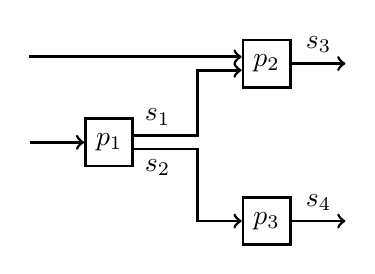
\begin{tikzpicture}[line width = 1pt,
                    process/.style    = {rectangle, draw, fill = white, minimum size = 0.6cm, inner sep = 0pt, align = center}
                    ]
    % \draw (0, 10) to[grid with coordinates] (18, 18);

    \node[process] (p1) at (0, 1) {$p_1$};
    \node[process] (p2) at (2, 2) {$p_2$};
    \node[process] (p3) at (2, 0) {$p_3$};

    \draw[<-] (p1) -- ++ (180:1cm);
    \draw[->] (p1.15) node[anchor = south west] {$s_1$} -- ++ (0:0.8cm) |- (p2.195);
    \draw[->] (p1.345) node[anchor = north west] {$s_2$}-- ++ (0:0.8cm) |- (p3);
    \draw[<-] (p2.165) -- ++ (180:2.7cm);
    \draw[->] (p2) -- ++ (0:1cm) node[anchor = south, midway] {$s_3$};
    \draw[->] (p3) -- ++ (0:1cm) node[anchor = south, midway] {$s_4$};;
\end{tikzpicture} 
    %\fi
  \end{center}
  \tabulinesep = 4pt
  \begin{tabu}to \textwidth{@{}X[-1, c]X|X[-1, c]X[-1]X[-1]@{}}
    \tabucline[1pt]{-}
    Symbol & Description      & Symbol & Description   & Value(\$)\\
    \hline
    $p_1$ & distillation      & $s_1$ & semi-product 1 & $10,000$\\
    $p_2$ & heating           & $s_2$ & semi-product 2 & $20,000$\\
    $p_3$ & mixing \& heating & $s_3$ & product 1      & $50,000$\\
          &                   & $s_4$ & product 2      & $70,000$\\
    \tabucline[1pt]{-} 
  \end{tabu}  
  \end{overlayarea} 
\end{frame}

\begin{frame}{Security Strategies}
  \begin{overlayarea}{\textwidth}{7cm}
  The security strategies are shown as follows.\vspace{10pt}

  \scriptsize
  \extrarowsep = 2mm
  \begin{tabu}to \textwidth{@{}X[-1, c, m]X[m]*2{X[-1, m]}@{}}
  \tabucline[1pt]{-}
  Symbol & Description & Prevented Attacks & Invalidated Functions\\
  \tabucline[1pt]{-}
  \only<+>{
    $m_{ 1}$ & shut down the web server              & $a_{3}$, $a_{4}$                       & ---      \\\hline
    $m_{ 2}$ & shut down the personal computer 1     & $a_{5}$                                & $f_{35}$ \\\hline
    $m_{ 3}$ & shut down the personal computer 2     & $a_{6}$                                & $f_{36}$ \\\hline
    $m_{ 4}$ & shut down the personal computer 3     & $a_{7}$                                & $f_{37}$ \\\hline
    $m_{ 5}$ & disconnect the security gateway 1     & $a_{8}$                                & $f_{38}$ \\\hline
    $m_{ 6}$ & shut down the data server 1           & $a_{10}$, $a_{11}$                     & $f_{38}$ \\\hline
    $m_{ 7}$ & shut down the engineer station 1      & $a_{12}$                               & $f_{41}$ \\\hline
    $m_{ 8}$ & encrypt the data amongst the PLC 1-4  & $a_{35}$, $a_{36}$, $a_{37}$, $a_{38}$ & ---      \\\tabucline[1pt]{-}
  }
  \only<+>{
    $m_{ 9}$ & disconnect the security gateway 2     & $a_{13}$                               & $f_{39}$ \\\hline
    $m_{10}$ & shut down the data server 2           & $a_{15}$, $a_{16}$                     & $f_{39}$ \\\hline
    $m_{11}$ & shut down the engineer station 2      & $a_{17}$                               & $f_{42}$ \\\hline
    $m_{12}$ & encrypt the data amongst the PLC 5-8  & $a_{39}$, $a_{40}$, $a_{41}$, $a_{42}$ & ---      \\\hline
    $m_{13}$ & disconnect the security gateway 3     & $a_{18}$                               & $f_{40}$ \\\hline
    $m_{14}$ & shut down the data server 3           & $a_{20}$, $a_{21}$                     & $f_{40}$ \\\hline
    $m_{15}$ & shut down the engineer station 3      & $a_{22}$                               & $f_{43}$ \\\hline
    $m_{16}$ & encrypt the data amongst the PLC 9-12 & $a_{43}$, $a_{44}$, $a_{45}$, $a_{46}$ & ---      \\\tabucline[1pt]{-}
  }
  \end{tabu}
  \end{overlayarea} 
\end{frame}

\begin{frame}{Recovery Strategies}
  \begin{overlayarea}{\textwidth}{7cm}
  The recovery strategies are shown as follows.\vspace{10pt}

  \scriptsize
  \extrarowsep = 2mm
  \begin{tabu}to \textwidth{@{}X[-1, c]X[-1]XX[-1, r]@{}}
  \tabucline[1pt]{-}
  Symbol & Description & Recovered Functions & Cost(\$) \\
  \tabucline[1pt]{-}
  \only<+>{  
    $n_{ 1}$ & reboot PLC1                           & $f_{4}$                                & $ 9,000$ \\\hline
    $n_{ 2}$ & reboot PLC2                           & $f_{7}$                                & $ 9,000$ \\\hline
    $n_{ 3}$ & reboot PLC3                           & $f_{8}$, $f_{9}$                       & $10,000$ \\\hline
    $n_{ 4}$ & reboot PLC4                           & $f_{5}$, $f_{6}$                       & $15,000$ \\\hline
    $n_{ 5}$ & reboot PLC5                           & $f_{14}$, $f_{15}$                     & $ 8,000$ \\\hline
    $n_{ 6}$ & reboot PLC6                           & $f_{18}$                               & $10,000$ \\\hline
    $n_{ 7}$ & reboot PLC7                           & $f_{19}$, $f_{20}$, $f_{21}$           & $ 2,000$ \\\hline
    $n_{ 8}$ & reboot PLC8                           & $f_{16}$, $f_{17}$                     & $13,000$ \\\tabucline[1pt]{-}
  }
  \only<+>{
    $n_{ 9}$ & reboot PLC9                           & $f_{30}$                               & $14,000$ \\\hline
    $n_{10}$ & reboot PLC10                          & $f_{25}$, $f_{33}$                     & $ 7,500$ \\\hline
    $n_{11}$ & reboot PLC11                          & $f_{27}$, $f_{28}$, $f_{29}$           & $14,000$ \\\hline
    $n_{12}$ & reboot PLC12                          & $f_{31}$, $f_{32}$                     & $11,000$ \\\tabucline[1pt]{-} 
  }
  \end{tabu}
  \end{overlayarea} 
\end{frame}